\documentclass[10.5pt]{article}
\usepackage{amsmath,amssymb,amsthm}
\usepackage{listings}
\usepackage{graphicx}
\usepackage[shortlabels]{enumitem}
\usepackage{tikz}
\usepackage[margin=1in]{geometry}
\usepackage{fancyhdr}
\usepackage{epsfig} %% for loading postscript figures
\usepackage{amsmath}
\usepackage{float}
\usepackage{amssymb}
\usepackage{caption}
\usepackage{subfigure}
\usepackage{graphics}
\usepackage{titlesec}
\usepackage{mathrsfs}
\usepackage{amsfonts}
\usepackage{indentfirst}
\usepackage{fontspec}

\renewcommand{\baselinestretch}{1.2}%Adjust Line Spacing
%\geometry{left=2.0cm,right=2.0cm,top=2.0cm,bottom=2.0cm}% Adjust Margins of the File
\usepackage{tikz-qtree}
\usetikzlibrary{graphs}
\tikzset{every tree node/.style={minimum width=2em,draw,circle},
	blank/.style={draw=none},
	edge from parent/.style=
	{draw,edge from parent path={(\tikzparentnode) -- (\tikzchildnode)}},
	level distance=1.2cm}
\setlength{\parindent}{0pt}
%\setlength{\parskip}{5pt plus 1pt}
\setlength{\headheight}{13.6pt}
\newcommand\question[2]{\vspace{.25in}\hrule\textbf{#1: #2}\vspace{.5em}\hrule\vspace{.10in}}
\renewcommand\part[1]{\vspace{.10in}\textbf{(#1)}}
\newcommand\algorithm{\vspace{.10in}\textbf{Algorithm: }}
\newcommand\correctness{\vspace{.10in}\textbf{Correctness: }}
\newcommand\runtime{\vspace{.10in}\textbf{Running time: }}
\pagestyle{fancyplain}
% Create horizontal rule command with an argument of height
\newcommand{\horrule}[1]{\rule{\linewidth}{#1}}
% Set the title here
\title{
	\normalfont \normalsize
	\textsc{ShanghaiTech University} \\ [25pt]
	\horrule{0.5pt} \\[0.4cm] % Thin top horizontal rule
	\huge CS101 Algorithms and Data Structures\\ % The assignment title
	\LARGE Fall 2020\\
	\LARGE Homework 1\\
	\horrule{2pt} \\[0.5cm] % Thick bottom horizontal rule
}
% wrong usage of \author, never mind
\author{}
\date{Due date: 23:59, September 14, 2020}

% set the header and footer
\pagestyle{fancy}
\lhead{CS101 Algorithms and Data Structures}
\chead{Homework 1}
\rhead{Due date: 23:59, September 14, 2020}
\cfoot{\thepage}
\renewcommand{\headrulewidth}{0.4pt}

% special settings for the first page
\fancypagestyle{firstpage}
{
	\renewcommand{\headrulewidth}{0pt}
	\fancyhf{}
	\fancyfoot[C]{\thepage}
}

% Add the support for auto numbering
% use \problem{title} or \problem[number]{title} to add a new problem
% also \subproblem is supported, just use it like \subsection
\newcounter{ProblemCounter}
\newcounter{oldvalue}
\newcommand{\problem}[2][-1]{
	\setcounter{oldvalue}{\value{secnumdepth}}
	\setcounter{secnumdepth}{0}
	\ifnum#1>-1
	\setcounter{ProblemCounter}{0}
	\else
	\stepcounter{ProblemCounter}
	\fi
	\section{Problem \arabic{ProblemCounter}: #2}
	\setcounter{secnumdepth}{\value{oldvalue}}
}
\newcommand{\subproblem}[1]{
	\setcounter{oldvalue}{\value{section}}
	\setcounter{section}{\value{ProblemCounter}}
	\subsection{#1}
	\setcounter{section}{\value{oldvalue}}
}

\setmonofont{Consolas}
\definecolor{blve}{rgb}{0.3372549 , 0.61176471, 0.83921569}
\definecolor{gr33n}{rgb}{0.29019608, 0.7372549 , 0.64705882}
\makeatletter
\lst@InstallKeywords k{class}{classstyle}\slshape{classstyle}{}ld
\makeatother
\lstset{language=C++,
	basicstyle=\ttfamily,
	keywordstyle=\color{blve}\ttfamily,
	stringstyle=\color{red}\ttfamily,
	commentstyle=\color{green}\ttfamily,
	morecomment=[l][\color{magenta}]{\#},
	classstyle = \bfseries\color{gr33n}, 
	tabsize=4
}


\begin{document}
	
	\maketitle
	\thispagestyle{firstpage}
	%\newpage
	\vspace{3ex}
	
	\begin{enumerate}
		\item Please write your solutions in English. 
		
		\item Submit your solutions to gradescope.com.  
		
		\item Set your FULL Name to your Chinese name and your STUDENT ID correctly in Account Settings. 
		
		\item If you want to submit a handwritten version, scan it clearly. Camscanner is recommended. 
		
		\item When submitting, match your solutions to the according problem numbers correctly. 
		
		\item No late submission will be accepted.
		
		\item Violations to any of the above may result in zero grade. 
	\end{enumerate}
	\newpage
	
  \question{1}{Academic integrity (10 pts)}
    
    Please determine who violated academic plagiarism in the following situations. A stands for Alice, B stands for Bob, N stands for None, AB stands for Both.
    	\begin{itemize}
    		\item[(a)]Alice and Bob are good friends, Alice asked if Bob could send her codes so that she could look at it(promising, of course, not copying). Then Bob sent his codes to Alice, Alice copied it and handled it in.
    		\item[(b)]Alice and Bob are roommates. Bob let Alice use his laptop to play PUBG, and Alice copied Bob's solution for assignment.
    		\item[(c)]Alice uses Bob's computer to complete the programming assignment and accidentally submits her own assignment using Bob's account. After that, Alice and Bob resubmitted their assignments using their own accounts.
    		\item[(d)]Bob is Alice's boyfriend. In order to promote feelings, they competed in the discussion room about who could complete the programming assignment first. There was no communication during the period.
    		\item[(e)]Alice found the homework question in CSDN and copied the answer on her homework.
    	\end{itemize}
	
	\pagebreak



	\question{2}{Array for list (10 pts)}
	In this question, we use two arrays: ``next" and ``value" to simulate a linked-list. 
	The elements at each index in ``next" and ``value" 
	are combined together to represent a node in the 
	linked-list, where ``next" represents the pointer 
	to the next node, and ``value" represents data in 
	the nodes.
	\begin{enumerate}[(a)]
		\item \textbf{Linked list from array representation (5 pts)}
		

		Here are the two arrays of ``next" and ``value".
		Please draw the linked list presented by the two arrays.
		\begin{center}
		\begin{tabular}{|c|c|c|c|c|c|c|c|c|c|c|c|}
			\hline
			index&0&1&2&3&4&5&6&7&8&9\\
			\hline
			value&A&B&C&D&E&F&G&H&I&J\\
			\hline
			next&7&5&3&9&/&2&0&1&4&8\\
			\hline

		\end{tabular}
			
	\end{center}
		\vspace{3cm}
		\item \textbf{Array representation for a linked list (5 pts)}
		 
		Fill in  the ``next" array in order to make the array and the linked-list showing below equivalent.

		\begin{center}
	
		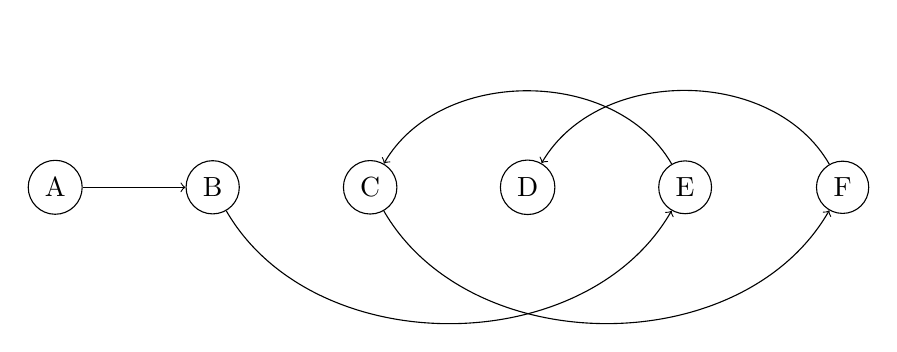
\begin{tikzpicture}
			\node[shape=circle,draw=black] (A) at (0,0) {A};
			\node[shape=circle,draw=black] (B) at (2,0) {B};
			\node[shape=circle,draw=black] (C) at (4,0) {C};
			\node[shape=circle,draw=black] (D) at (6,0) {D};
			\node[shape=circle,draw=black] (E) at (8,0) {E};
			\node[shape=circle,draw=black] (F) at (10,0) {F};
		
			\path [->](A) edge node {} (B);
			\path [->](B) edge[bend right=60] node {} (E);
			\path [->](E) edge[bend right=60] node {} (C);
			\path [->](F) edge[bend right=60] node {} (D);
			\path [->](C) edge[bend right=60] node {} (F); 
		\end{tikzpicture}
	\end{center}
		
	\begin{center}
		\begin{tabular}{|c|c|c|c|c|c|c|c|c|}
			\hline
			index&0&1&2&3&4&5\\
			\hline
			value&A&B&C&D&E&F\\
			\hline
			next&&&&&&\\
			\hline

		\end{tabular}
			
	\end{center}

	\end{enumerate}

	\pagebreak

	%------------------------------------------------------------------
	\question{3}{List operations (10 pts)}
	
	You should use the defined linked list to implement all the newly defined operations. Please pay attention to the following rules:
	\begin{enumerate}
		\item There is no dummy node as the entry node, i.e. if the linked list is not empty, 
		\texttt{head} points to the first node,
		\texttt{tail} points to the last node.
		\item Use \texttt{new} and \texttt{delete} to deal with memory issues.
		\item Remember to maintain \texttt{head} and \texttt{tail}.
		\item You may not use all of the blank lines. There is at most one statement (ended with \texttt{;}) in each blank line.
		\item For simplicity, the retrieve function is not given and you can directly use the private attributes like \texttt{node->data}, \texttt{list->head} etc. (Invalid for programming but OK for this homework)
		\item If there is any syntax error, this line will be counted as wrong.
	\end{enumerate}
	
	\hrulefill
	
	\begin{lstlisting}[language=C++,moreclass={Node}]
class Node {
public:
	int data;
	Node * next;
	
	Node(int val, Node * nextNode): data(val), next(nextNode)
	{
	}
	... ...
};
Node * head;
Node * tail;
	\end{lstlisting}    
	
	\begin{enumerate}[(a)]
		\item \textbf{Insert before (5 pts)}
		
		This operation has been discussed in detail  in the lecture slides. Given a new data and a target node, create a new node using the new data and insert it before the target node. You should implement this function with $O(1)$ time complexity.
		\begin{enumerate}
			\item[$\bullet$] Assume the target node is neither \texttt{head} nor \texttt{tail}.
		\end{enumerate}
		
		\hrulefill
		\begin{lstlisting}[language=C++,moreclass={Node}]
void InsertBefore(Node * curr, int data)
{
	Node * newNode = new Node(___________________________);
	
	______________________________________________________;
	
	______________________________________________________;
}
		\end{lstlisting}
		\item \textbf{Reverse (5 pts)}
		
		Now think about how to reverse a list.
		Given \texttt{head} and \texttt{tail} of a non-empty list,
		\begin{enumerate}
			\item[$\bullet$] Assume the list is not empty.
		\end{enumerate}
		\hrulefill
		\begin{lstlisting}[language=C++,moreclass={Node}]
void Reverse(Node * &head, Node * &tail) {
		
	Node * prevNode = head;
	
	Node * rotateNode = _____________________;
	
	head->next = NULL;
	
	while (rotateNode) {
		
		Node *next = rotateNode->next;
		
		_____________________________________;
		
		_____________________________________;
		
		rotateNode = next;
		
	}
	
	swap(head, tail);
	
}
		\end{lstlisting}
		
		\item \textbf{[ Bonus ] Is there a cycle? (0 pts)}
		
		Sometimes, a list may form a cycle, which means its tail is pointing at 
		a node in the list  instead of \texttt{NULL}.
		
		$$
		\begin{aligned}
		A \rightarrow B \rightarrow C& \rightarrow D \rightarrow E\rightarrow &F\\
		\uparrow&&\downarrow\\
		J&\leftarrow I\leftarrow H\leftarrow&G
		\end{aligned}
		$$
		
		Since the list may be extremely large, it is not allowed to record whether a
		node is visited -- which means you could not use extra space bigger other than $O(1)$.
		Given the head of a list, describe how to determine if there is a cycle on the list.
		
		(Note: tail and length are not given. 
		If there is no cycle on the list, 
		the last node is supposed to 
		be pointing at \texttt{NULL})		

		(Hint: Think about 3000 meters long run in the playground.)

	\end{enumerate}
	
	\pagebreak
	
\end{document}